\chapter{Generování fraktálů}\label{chapter:generovani-fraktalu}

V této poslední kapitole navážeme na znalosti z~kapitoly předchozí, tj. č.~\ref{chapter:klasifikace-fraktalu}. Proto zde opět čtenáři doporučuji se podívat na její obsah (vyjma sekcí týkajících se matematického základu). Podíváme se stručný teoretický rozbor algoritmů pro generování fraktálních útvarů, i na jejich praktickou implementaci. Než tak však učiníme, uděláme si krátké povídání o~způsobu, jakým budeme rozbory vůbec provádět.

Vzorový způsob implementace všech zde zmíněných algoritmů lze nalézt v~přiloženém programu.

\section{Stručně k zápisu programů}\label{sec:zapis-programu}

V době psaní tohoto textu existuje mnoho programovacích jazyků\index{jazyk!programovací}\index{programovací jazyk} a nejspíše lze bezpečně předpokládat, že budou přibývat další. Nikoho tak nejspíše nepřekvapí, že vzhledem k současnému (dosti rychlému) vývoji v oblasti informatiky mnoho jazyků, které dříve byly považovány za nové a inovativní, postupně zastaraly a jiné pro mnoho jedinců dokonce upadly v zapomnění. Avšak jiné naopak si svoji pozici drží dodnes. Pro účely tohoto textu byl v rámci praktických ukázek, které uvidíte, zvolen jazyk \textbf{Python}\index{Python}, neboť jeho syntaxe není složitá\footnote{Složitost programovacího jazyka je, z pochopitelných důvodů, dosti subjektivní pojem, neboť závisí i na zkušenostech programátora.} a zároveň tak není příliš obtížné si v mnoha případech domyslet význam jednotlivých příkazů\footnote{Samozřejme nelze v tomto ohledu mluvit za každého (potenciálního) čtenáře. Pokud by tak kdykoliv vznikla nějaká nejasnost ohledně významu použitých příkazů, lze se podívat na stránky oficiální dokumentace jazyka Python: \url{https://docs.python.org}}. Zároveň však poznamenejme, že stejně jako v případě matematické části tohoto textu, i zde budeme pracovat s předpokladem, že čtenář je seznámen se základními koncepty programování a algoritmizace všeobecně. Nebudeme se zde tedy řešit, co je to proměnná\index{proměnná}, pole\index{pole} (resp. v Pythonu seznamem\index{seznam}), funkce, podmínky aj.

Zároveň bychom neměli zapomínat na zájemce používající jiné programovací jazyky. Proto kromě praktických ukázek si prezentované algoritmy uvedeme i pomocí tzv. \emph{pseudokódu}\index{pseudokód}. Pseudokód nepředstavuje sám o sobě žádnou formu programovacího jazyka. Jedná se čistě o abstraktní popis psaný především pro člověka, který lze však s minimálním úsilím přepsat do libovolného programovacího jazyka. Jednoduchým příkladem pseudokódu je např. \ref{alg:ukazka-pseudokodu}.
\begin{algorithm}
    \KwIn{Seznam čísel $x_1,x_2,\ldots,x_n$.}
    $\text{max}\gets x_1$\\
    \For{$i=1,2,\ldots,n$}{
        \If{$x_i>\textup{max}$}{
            $\textup{max}\gets x_i$
        }
    }
    \Return{\textup{max}}
    \caption{Ukázkový pseudokód (hledání minima)}
    \label{alg:ukazka-pseudokodu}
\end{algorithm}
Implementace takového algoritmu např. právě v jazyce Python si čtenář může prohlédnout u programu \ref{prog:ukazka-implementace-pseudokodu}.
\begin{program}[h]
    \begin{lstlisting}[style=python]
def findMax(numbers: list) -> int:
    maximum = numbers[0]
    for i in range(len(numbers)):
        number = numbers[i]
        if number > maximum:
            maximum = number
    return maximum
    \end{lstlisting}
    \caption{Možná implementace algoritmu \ref{alg:ukazka-pseudokodu}}
    \label{prog:ukazka-implementace-pseudokodu}
\end{program}
Pochopitelně se v konkrétní implementaci mohou vyskytovat různé odchylky. Např. v programu \ref{prog:ukazka-implementace-pseudokodu} využíme proměnnou \texttt{number}, kterou bychom jistě mohli vypustit a pracovat přímo se seznamem \texttt{numbers}, tzn. \texttt{numbers[i]}. Nebo bychom například nemuseli program vůbec zapisovat jako funkci, či bychom mohli např. jinak pojmenovat proměnné. To jsou však v celkovém kontextu pouhé drobnosti. V rámci textu se ovšem budeme snažit držet jednotné konvence, tedy že programy budeme vždy psát jako funkce/procedury a proměnné budeme pojmenovávat vždy v angličtině, neboť je to při programování zkrátka zvyklost.
\section{Implementace L-systémů a želví grafiky}\label{sec:implementace-lsystemu-a-zelvi-grafiky}

Na základní princip L-systémů\index{L-systém} jsme se podívali v části \ref{sec:L-systemy}. Jejich implementace je do jisté míry přímočará. Řešení je potřeba rozdělit na dvě části: implementace \emph{samotného L-systému} a \emph{želví grafiky}\index{želví grafika}.

\subsection{Implementace L-systémů}\label{subsec:implementace-lsystemu}

L-systém nepředstavuje nikterak složitou matematickou strukturu. Z definice (viz \ref{def:lsystem}) je potřeba znát pouze používané \emph{neterminály}\index{neterminál}, \emph{axiom}\index{axiom} a seznam přepisovacích pravidel. O to jednodušší je situace, započítáme-li fakt, že neterminální symboly (resp. jejich význam) v případě námi používaných L-systémů jsou pevně dané, tedy není třeba je explicitně uvádět v definici. L-systém lze tak implementovat jako jednoduchou třídu s atributy \texttt{word} obsahující aktuální slovo po $k$-té iteraci a slovník pravidel \texttt{rules} (viz program \ref{prog:konstruktor-lsystem}).
\begin{program}[h]
    \begin{lstlisting}[style=python]
class LSystem:
    def __init__(self, axiom: str, rules: dict) -> None:
        self._word = axiom
        self._rules = rules
\end{lstlisting}
    \caption{Konstruktor třídy pro L-systém}
    \label{prog:konstruktor-lsystem}
\end{program}
Slovní pravidel \texttt{rules} má jednoduchou strukturu. Klíče tvaří levé strany pravidel a k nim přiřazené hodnoty naopak tvoří pravé strany pravidel. Jeho vzhled může vapadat např. takto:
\begin{verbatim}
rules = {
    "X": "F-[[X]+X]+F[+FX]-X",
    "F": "FF"
}
\end{verbatim}
Poměrně zásadní pro nás však bude především metoda pro aplikaci jednotlivých pravidel. Pro další výklad si však zavedeme pohodlnější zápis řetězců, který je v programování zcela běžný.
\begin{definition}\label{def:index-retezce}
    Nechť $\alpha=x_1x_2\ldots x_n$ je slovo nad libovolnou abecedou $\Sigma\neq\emptyset$. Pak pro každé $1\leqslant i\leqslant n$ definujeme $\alpha[i]=x_i$.
\end{definition}
Myšlenka je velice intuitivní. Obecně máme-li řetězec $w$ po $m$-té iteraci a množinu přepisovacích pravidel $P\subseteq\set{a\to\alpha\mid a\in V,\;\alpha\in V^*}$, kde $V$ je abeceda, pak stačí pro každý znak $w[i]$, kde $1\leqslant i\leqslant n$, pouze zkontrolovat, zda není na levé straně nějakého pravidla v $P$. Pokud ano, dojde k aplikaci příslušného pravidla\footnote{Technicky vzato jsme z formálních důvodů v definici L-systému \ref{def:lsystem} přidali i pravidla tvaru $a\to a$, aby nedošlo k situaci, že pro $a$ neexistuje pravidlo. Avšak z hlediska prakticné implementace toto není překážkou, neboť v případě absence takového pravidla jednoduše symbol přeskočíme.}. Viz pseudokód \ref{alg:iterace-slova-lsystem}.
\begin{algorithm}[h]
    \KwIn{Množina pravidel $P$, slovo $w$, číslo $k\in\N$}
    $w^\prime\gets\lambda$\\
    \For{$m=1,2,\ldots,k$}{
        \For{$i=1,2,\ldots,|w|$}{
            \If{\textup{existuje pravidlo tvaru $(w[i]\to\alpha)\in P$}}{
                $w^\prime\gets w^\prime[1]\dots w^\prime[i-1]\alpha$
            }
            \Else{
                $w^\prime=w^\prime w[i]$
            }
        }
    }
    \Return{$w^\prime$}\\
    \KwOut{Slovo $w^\prime$ odvozené po $k$ iteracích ze slova $w$}
    \caption{Algoritmus pro $k$-tou iteraci slova $w$}
    \label{alg:iterace-slova-lsystem}
\end{algorithm}
Implementace je, vzhledem k dostupným funkcím v Pythonu, až překvapivě jednoduchá. O tom se čtenář může přesvědčit sám v případě kódu \ref{prog:iterace-slova-lsystem}.
\begin{program}[h]
\begin{lstlisting}[style=python]
def iterate(self, iteration_count: int) -> None:
    for _ in range(iteration_count):
        self._word = self._word.translate(str.maketrans(self._rules))
\end{lstlisting}
    \caption{Implementace algoritmu \ref{alg:iterace-slova-lsystem}.}
    \label{prog:iterace-slova-lsystem}
\end{program}
Pojďme si stručně rozebrat použíté funkce, resp. metody, v programu \ref{prog:iterace-slova-lsystem}.
\begin{itemize}
    \item \texttt{str.maketrans} vytvoří ze zadaného slovníku překladovou tabulku pro metodu \texttt{translate}. Její struktura odpovídá slovníku obsahující dvojice \emph{(Unicode\index{Unicode} hodnota, znak)}
    \item \texttt{translate} nahradí každý ze znaků řetězcem uvedeným v překladové tabulce.
\end{itemize}
Tímto způsobem lze implementovat třídu, kde vygenerujeme příslušný řetězec, který následně budeme interpretovat pomocí želví grafiky\index{želví grafika}.

\subsection{Implementace želví grafiky}\label{subsec:implementace-zelvi-grafiky}

Druhou částí je naprogramování želví grafiky. Nyní pracujeme se scénářem, že máme vygenerovaný příslušný řetězec znaků $w$, jehož znaky chceme interpretovat. Za účelem jednoduchosti se pokusíme striktně oddělit samotnou \emph{geometrickou interpretaci řetězce} od jeho \emph{grafické interpretace}.

Pro připomenutí významů jednotlivých symbolů doporučuji se znovu podívat do tabulek \ref{table:vyznam-symbolu-zelva} a \ref{table:vyznam-symbolu-zelva-zasobnik}. Nejdříve si však ujasněme, jaké informace si potřebujeme o želvě uchovávat.
\begin{itemize}
    \item Vzdálenost $d$, o kterou se želva při každém kroku posune,
    \item aktuální pozice želvy $(x,y)$,
    \item úhel $\alpha\in\langle 0,2\pi)$ udávající směr želvy
    \item přírůstek úhlu $\delta$,
    \item seznam nakrelených úseček reprezentované jako uspořádané čtveřice
    \[(x_0,y_0,x_1,y_1),\]
    kde $(x_0,y_0)$ a $(x_1,y_1)$ jsou souřadnice počátečního, resp. koncového bodu.
\end{itemize}
Podobně jako v případě L-systému, i zde můžeme želvu reprezentovat jako třídu (viz program \ref{prog:konstruktor-zelva}).
\begin{program}[h]
\begin{lstlisting}[style=python]
class Turtle:
    def __init__(self, step: float, position: Vector = Vector(0, 0), angle: float = 0) -> None:
        self._position = position
        self._step = step
        self._angle = (angle % 360) * math.pi / 180
        self._pen_down = False
        self._lines = []

        self._x_min, self._y_min = position.x, position.y
        self._x_max, self._y_max = position.x, position.y
\end{lstlisting}
    \caption{Konstruktor třídy pro želvu}
    \label{prog:konstruktor-zelva}
\end{program}

V tomto případě zvolíme při implementaci želvy následující strategii. Představíme si ji tak, že na sobě připevněné pero a budeme si pouze pamatovat, zda je či není v danou chvíli položeno na plátně. Pokud ano a želva provede krok vpřed, nakreslí za sebou úsečku.

Všechny atributy jsou vysvětleny níže.
\begin{itemize}
    \item \texttt{self.\_position} uchovává pozici želvy $(x,y)$,
    \item \texttt{self.\_step} reprezentuje velikost kroku $d$,
    \item \texttt{self.\_angle} je počáteční úhel otočení želvy přepočítaný v radiánech,
    \item \texttt{self.\_pen\_down} udává, zda je pero položeno na plátně.
    \item \texttt{self.\_lines} ukládá seznam dosud nakrelených úseček.
\end{itemize}
V konstruktoru třídy \texttt{Turtle} se navíc nachází soukromé atributy \texttt{self.\_x\_min}, \texttt{self.\_x\_max}, \texttt{self.\_y\_min} a \texttt{self.\_y\_max}. Ty nám budou sloužit pro pozdější vykreslování výsledného útvaru. Průběžně si v nich budeme uchovávat minimální, resp. maximální, souřadnici $x$ a $y$ ze všech dosud vygenerovaných úseček.
\section{Implementace IFS}\label{sec:implementace-ifs}

Systémy iterovaných funkcí a~k nim související teorii jsme si vyložili již v~části \ref{sec:ifs}. Podobně jako v~případě L-systémů,~i zde budeme postupovat přímo z~definice. Konkrétně jsme si definovali IFS jako množinu kontrakcí
\[\set{\mapping{\psi_i}{X}{X}\mid 1\leqslant i~\leqslant n},\]
přičemž jsme následně zkoumali a~pracovali se zobrazením $\Psi$ daným předpisem
\[\Psi(B)=\bigcup_{i=1}^n\psi_i(B)\;,\;B\in\hyperspace(X).\]
O zobrazení $\Psi$ jsme následně dokázali,~že se též jedná o~kontrakci (viz věta \ref{thm:sjednoceni-kontrakci}).

Konkrakce,~s nimiž jsme pracovali,~byla tzv. \emph{afinní zobrazení}\index{zobrazení!afinní}\index{afinní zobrazení} v~$\R^2$,~tedy jejich předpis byl ve tvaru
\begin{equation}\label{eq:afinni-zobrazeni}
    f(x,y)=\left(\begin{matrix}
        a~& b\\
        c & d
    \end{matrix}\right)\left(\begin{matrix}
        x\\
        y
    \end{matrix}\right)+\left(\begin{matrix}
        e\\
        f
    \end{matrix}\right)=\left(\begin{matrix}
        ax+by+e\\
        cx+dy+f
    \end{matrix}\right).
\end{equation}
V konečném důsledku si tedy stačilo uchovat pouze koeficienty $a,b,\ldots,f$. A~toho přesně využijeme i~zde. Daná afinní zobrazení budeme reprezentovat seznamem uspořádaných šestic
\[(a,b,c,d,e,f).\]
Dále potřebujeme již pouze znát počáteční obrazec. Ačkoliv bychom mohli jistě různými sofistikovanými způsoby reprezentovat celou řadu množin,~my se omezíme pouze na mnohoúhelníky\footnote{V konečném důsledku,~jak již víme z~Banachovy věty \ref{thm:banach},~počáteční obrazec nehraje žádnou roli pro atraktor zobrazení $\Psi$.},~neboť jejich reprezentace je velmi jednoduchá. Stačí si pamatovat pozice jeho vrcholů
\[(x_1,y_1),(x_2,y_2),\ldots,(x_n,y_n).\]
I zde provedeme implementaci IFS pomocí třídy (viz ukázka \ref{prog:konstruktor-ifs}).
\begin{program}[h]
\begin{lstlisting}[style=python]
from copy import deepcopy

class IFS:

    def __init__(self,~starting_figure: list,~tr_coefs: list = []) -> None:
        self._figures = [starting_figure]
        self._total_iterations = 0

        # Min/max coordinates (used for centering)
        self._x_min,~self._y_min,~self._x_max,~self._y_max = 0,~0,~0,~0
        self.__update_min_max_coords()

        self._transformations = set()
        for tpl in tr_coefs:
            def transformation(point,~tpl=deepcopy(tpl)):
                return Vector(
                    tpl[0]*point.x + tpl[1]*point.y + tpl[4],
                    tpl[2]*point.x + tpl[3]*point.y + tpl[5]
                )
            self._transformations.add(transformation)
    
    
    def __update_min_max_coords(self) -> None:
        self._x_min = min(point.x for figure in self._figures for point in figure)
        self._y_min = min(point.y for figure in self._figures for point in figure)
        self._x_max = max(point.x for figure in self._figures for point in figure)
        self._y_max = max(point.y for figure in self._figures for point in figure)
\end{lstlisting}
    \caption{Konstruktor pro třídu \texttt{IFS}}
    \label{prog:konstruktor-ifs}
\end{program}
Po vzoru třídy \texttt{Turtle},~kterou jsme si ukázali v~minulé sekci \ref{sec:implementace-lsystemu-a-zelvi-grafiky} i~zde si budeme průběžně aktualizovat minimální a~maximální hodnoty souřadnic pro pozdější manipulaci s~obrazcem. Dále zde máme dvojici důležitých atributů:
\begin{itemize}
    \item \texttt{self.\_figures} uchovává všechny vygenerované obrazce po obecně $k$-té iteraci jako seznam uspořádaných $n$-tic vrcholů.
    \item \texttt{self.\_transformations} ukládá zadané kontrakce $\psi_1,\psi_2,\ldots,\psi_m$ jako first-class funkce\index{first-class funkce}\index{funkce!first-class}. Výpočet probíhá podle \eqref{eq:afinni-zobrazeni}.
\end{itemize}
Co je to \emph{first-class funkce}\footnote{Též se lze někdy setkat s~českým označením funkce nebo obecněji objekty \emph{první kategorie}\index{objekty první kategorie}\index{funkce první kategorie}\index{funkce!první kategorie}.}\index{first-class funkce}\index{funkce!first-class}? Jedná se o~koncept práce s~funkcemi jakožto standardními objekty,~na které se lze odkazovat. V~praxi to znamená možnost předávat funkce jako parametry,~používat je jako návratové hodnoty,~nebo ukládat je do proměnných. To se nám v~tomto případě velmi hodí,~neboť tyto funkce potřebujeme vytvářet až za běhu programu v~závislosti na zadaných koeficientech afinních zobrazení.

V této části se zaměříme pouze na generování výsledného obrazce v~jednotlivých iteracích. V~tomto ohledu bude potřeba si uchovávat nově vygenerované útvary do nějaké struktury. To vše je shrnuto v~algoritmu \ref{alg:iterace-ifs}.
\begin{algorithm}[h]
    \KwIn{IFS $\set{\psi_1,\ldots,\psi_n}$,~množina útvarů $\mathcal{F}$,~číslo $k\in\N$}
    \For{$i=1,2,\ldots,k$}{
        $\mathcal{F}^\prime\gets\emptyset$\;
        \ForEach{$F\in\mathcal{F}$}{
            \ForEach{$\psi\in\set{\psi_1,\ldots,\psi_n}$}{
                $\mathcal{F}^\prime\gets\mathcal{F}^\prime\cup\set{\psi(F)}$\;
            }
        }
        $\mathcal{F}\gets \mathcal{F}^\prime$\;
    }
    \Return{$\mathcal{F}$}\;
    \KwOut{Nová množina útvarů $F$}
    \caption{$k$-tá iterace IFS}
    \label{alg:iterace-ifs}
\end{algorithm}
Speciálně,~pokud bychom chtěli vygenerovat $k$-tou z~počátečního obrazce $F_0$,~stačí algoritmus zavolat na množinu $\set{F_0}$. Praktickou implementaci si lze prohlédnout v~ukázce \ref{prog:iterace-ifs}.
\begin{program}[h]
\begin{lstlisting}[style=python]
def iterate(self,~iterations: int) -> None:
    for _ in range(iterations):
        figures_new = []
        
        for figure in self._figures:
            for tr in self._transformations:
                figure_new = []
                for point in figure: figure_new.append(tr(point))

                figures_new.append(figure_new)
    
        self._figures = figures_new
\end{lstlisting}
    \caption{Implementace algoritmu \ref{alg:iterace-ifs} ve třídě \texttt{IFS}}
    \label{prog:iterace-ifs}
\end{program}
Posunutí obrazce na střed si již může čtenář samostatně rozmyslet. Provedení by však bylo obdobné jako v~případě L-systémů.
\section{Implementace Time Escape algoritmů}\label{sec:implementace-tea}

Poslední kategorii fraktálních útvarů tvořily tzv. \emph{Juliovy množiny}, u nichž jsme si jednoduše vysvětlili, že jejich generování probíhá pomocí tzv. \emph{Time Escape algoritmů}\index{Time Escape algoritmus}\index{algoritmus!Time Escape}. Jejich princip lze nastínit následovně: na vstupu zadáme nějakou komplexní polynomiální funkci $f$ a dále čísla $m\in\N_0$ a $r\in\R$. Čislo $m$ bude sloužit jako horní hranice počtu iterací, který pro každý bod v určitě omezené oblasti komplexní roviny provedeme (to lze pochopitelně dospecifikovat, avšak teď to není úplně podstatné). Pokud v kterékoliv iteraci nastane, že $|f^{\circ k}(z)|>r$, pak bod vyloučíme ze zkoumané množiny. Naopak v případě, že pro každé $0\leqslant k\leqslant m$ je $|f^{\circ k}(z)|\leqslant r$, pak prohlásíme, že bod náleží Juliově množině.

\subsection{Aproximace vyplněné Juliovy množiny}\label{subsec:aproximace-vyplnene-juliovy-mnoziny}

Podívejme se na tento algoritmus trochu blíže v pseudokódu \ref{alg:generovani-vyplnene-jf}.
\begin{algorithm}
    \KwIn{Komplexní polynomiální funkce $f$, maximální počet iterací $m\in\N_0$, číslo $r\in\R$, konečné množiny $X\subset\langle x_{\text{min}},x_{\text{max}}\rangle$ a $Y\subset\langle y_{\text{min}},y_{\text{max}}\rangle$}
    $K\gets\emptyset$\;
    \ForEach{\textup{$(a,b)\in X\times Y$}}{
        $z\gets a+b\imag$\;
        $t\gets\id$\;
        \For{$k=0,1,\ldots,m$}{
            $t\gets t\circ f$\;
            \If{$|t(z)|>r$}{
                pokračuj další iterací vnějšího cyklu\;
            }
        }
        $K\gets K\cup\set{z}$\;
    }
    \Return{$K$}\;
    \KwOut{Aproximace vyplněné Juliovy množiny $K(f)$}
    \caption{Generování vyplněné Juliovy množiny při pevném počtu iterací}
    \label{alg:generovani-vyplnene-jf}
\end{algorithm}
Nejspíše nikoho nepřekvapí, že při vyšších hodnotách čísla $m$ obdržíme lepší odhad Juliovy množiny příslušné polynomiální funkci $f$. Avšak vždy je potřeba zvážit náročnost výpočtu.

Znázornění (vyplněné) Juliovy množiny lze provést různými způsoby. Prezentovaný algorimus \ref{alg:generovani-vyplnene-jf} pouze určuje pro každý zvolený bod $z$, zda naleží, či nenáleží množině $J$. Avšak čtenář zajímající se o tuto partii matematiky již nejspíše viděl poměrně známý způosb vyobrazení těchto množin s barevným rozlišováním bodů. Tuto záležitost jsme již zmínili ke konci části \ref{subsec:juliovy-fatouovy-mnoziny}, avšak jeho podstatné aspekty jsou především algoritmické povahy a tedy teprve v této kapitole je více rozvedeme. K tomu se však dostaneme později.

Praktická implementace Time Escape algoritmů bude podstatně složitější, neboť si musíme vypořádat s konverzí samotného polynomu a rovněž vyřešit způsob vzorkování vybrané části komplexní roviny. Dále se budeme držet realizace pomocí třídy (viz ukázka \ref{prog:konstruktor-tea}).
\begin{program}[h]
\begin{lstlisting}[style=python]
class TEA:
    def __init__(self, width: int, height: int, sequence: str, step: int = 1, escape_radius: int = 2, bounds: tuple, var: str, explore_var: str):
        self._x_count, self._y_count = width // step, height // step
        
        self._iter_counts = [[0 for _ in range(self._x_count)] for _ in range(self._y_count)]
        self._width, self._height = width, height
        self._sequence = sequence
        self._var = var
        self._explore_var = explore_var
        self._total_iterations = 0
        self._escape_radius = escape_radius

        x_min, x_max, y_min, y_max = bounds

        x_vals = [x_min + step * (x_max - x_min) * j / width for j in range(self._x_count + 1)]
        y_vals = [y_min + step * (y_max - y_min) * i / height for i in range(self._y_count + 1)]
        self._complex_grid = [[x + 1j * y for x in x_vals] for y in y_vals]

        self._point_last_values = [[0 for _ in range(self._x_count)] for _ in range(self._y_count)]
\end{lstlisting}
    \caption{Konstruktor třídy \texttt{TEA}}
    \label{prog:konstruktor-tea}
\end{program}
Pojďme si konstruktor \ref{prog:konstruktor-tea} opět rozebrat.
\begin{itemize}
    \item \texttt{self.\_x\_count} a \texttt{self.\_y\_count} udávají počet bodů, které budeme prozkoumávat, ve směru reálné a imaginární osy. Jejich hodnoty jsou závislé na velikosti kroku \texttt{step}, kterou konstruktor přijímá jako parametr. Tedy např. s krokem $1$ v rámci intervalu $\langle-1,2\rangle$ budeme zkoumat celkem 4 body.
    \item V seznamu \texttt{self.\_iter\_counts} si budeme pro každý bod uchovávat, kolik iterací zadané funkce bylo potřeba, než posloupnost začala divergovat (tedy $|f^{\circ k}(z)|>r$). Ten využijeme především později při určování barev jednotlivých bodů.
    \item \texttt{self.\_sequence} uchovává předpis polynomální funkce, kterou budeme iterovat, jako řetězec. Předpisy budeme zadávat standardní syntaxí v Pythonu, tzn. např. pro Mandelbrotovu množinu, kde $f_c(z)=z^2+c$, bychom předpis napsali
    \begin{center}
        \texttt{z**2 + c}.
    \end{center}
    Levou stranu "\texttt{f(z) =}" pochopitelně psát netřeba.
    \item \texttt{self.\_var} udává, která proměnná v \texttt{self.\_sequence} je argumentem zadané funkce (typicky \texttt{z}).
    \item \texttt{self.\_explore\_var} uchovává proměnnou, za níž budeme dosazovat hodnoty zkoumaných bodů. Pro Juliovy množiny se typicky jedná přímo o argument zadané funkce $f$, ale např. pro Mandelbrotovu množinu je to \texttt{c}.
    \item \texttt{self.\_escape\_radius} reprezentuje číslo $r$, tedy hranici absolutní hodnoty čísla $z$, po jejímž překročení prohlásíme posloupnost iterací za divergentní.
    \item Parametr \texttt{bounds} specifikuje část komplexní roviny, z niž budeme zkoumat vybrané body. Jedná se o datový typ \texttt{tuple}, v našem případě uspořádanou čtveřici $(x_{\text{min}},x_{\text{max}},y_{\text{min}},y_{\text{max}})$.
    \item \texttt{self.\_complex\_grid} uchovává všechny body ze zadané části komplexní roviny jako komplexní čísla, tedy v Pythonu datový typ \texttt{complex}.
    \item Do seznamu \texttt{self.\_point\_last\_values} budeme ukládat hodnoty $f^{\circ k}(z)$ pro zadané $z$, kde $k$ je číslo poslední prozkoumané iterace (tzn. buď jsme u bodu prozkoumali maximální počet zadaných iterací, nebo výpočet skončil dříve kvůli překročení povolené absolutní hodnoty).
\end{itemize}
Je vidět, že atributů zde máme poměrně hodně. Zkusme si tedy nejdříve vyjasnit, jak bychom mohli pomocí těchto informací implementovat algoritmus pro iterování zadané polynomiální funkce. Již jsme si uvedli asi nejjednodušší možnost v rámci algoritmu \ref{alg:generovani-vyplnene-jf}. Jak by se ale situace změnila, když si budeme uchovávat počty iterací, které proběhly než jsme překročili zadanou absolutní hodnotu $r$ nebo dosáhli maximálního počtu $m$? Označme si takové pole např. $T$. Podívejme se na algoritmus \ref{alg:generovani-vyplnene-jf-pole}.
\begin{algorithm}[h]
    \KwIn{Komplexní polynomiální funkce $f$, maximální počet iterací $m\in\N_0$, číslo $r\in\R$, konečné množiny $X\subset\langle x_{\text{min}},x_{\text{max}}\rangle$ a $Y\subset\langle y_{\text{min}},y_{\text{max}}\rangle$}
    $K\gets\emptyset$\;
    Vytvoř prázdné pole $T$\;
    \ForEach{$(x,y)\in X\times Y$}{
        $z\gets x+y\imag$\;
        $t\gets\id$\;
        \For{$k=0,1,\ldots,m$}{
            $t\gets t\circ f$\;
            $T[x,y]\gets k$\;
            \lIf{$|t(z)|>r$}{opusť cyklus}
        }
        \lIf{$T[x,y]=m$}{$K\gets K\cup\set{z}$}
    }
    \Return{$K$}\;
    \KwOut{Aproximace vyplněné Juliovy množiny $K$}
    \caption{Generování vyplněné Juliovy množiny pomocí pole iterací $T$}
    \label{alg:generovani-vyplnene-jf-pole}
\end{algorithm}
Pro implementaci algoritmu \ref{alg:generovani-vyplnene-jf-pole} si však budeme muset rozmyslet, jak budeme pomocí řetězce s předpisem pro funkci $f$ (tj. atributu \texttt{self.\_sequence}) počítat její funkční hodnoty. Jistě se nabízí možnost vytvořit funkci pro vyhodnocení obecného matematického výrazu. Ač se jedná o poměrně hezké programovací cvičení a čtenář si jej může vyzkoušet, my si poradíme trochu jinak -- funkcí \texttt{eval}. Funkce \texttt{eval} jednoduše vyhodnotí zadaný výraz a za proměnné dosadí hodnoty podle slovníku poskytnutého v příslušném parametru/parametrech.

Tím se nám situace podstatně zlehčuje. Implementaci si může čtenář prohlédnout v ukázce \ref{prog:generovani-vyplnene-jf-pole}.
\begin{program}[h]
\begin{lstlisting}[style=python]
def iterate(self, iterations: int) -> None:
    for i in range(self._y_count):
        for j in range(self._x_count):
            # Initialize variables
            vars_dict = {self._var: 0, self._explore_var: self._complex_grid[i][j]}

            # Iterate
            for k in range(1, iterations + 1):
                try:
                    # Evaluate the next value in the sequence
                    vars_dict[self._var] = eval(self._sequence, {"math": math}, vars_dict)

                    # Check for escape condition
                    self._iter_counts[i][j] = k
                    if abs(vars_dict[self._var]) > self._escape_radius:
                        break
                except OverflowError:
                    self._iter_counts[i][j] = k
                    break
            
            self.point_last_values[i][j] = vars_dict[self._var]
\end{lstlisting}
    \caption{Implementace algoritmu \ref{alg:generovani-vyplnene-jf-pole}}
    \label{prog:generovani-vyplnene-jf-pole}
\end{program}

\subsection{Aproximace Juliovy množiny}\label{subsec:aproximace-juliovy-mnoziny}

S množinou $\filledinjulia(f)$ se rovněž pojí i její hranice $\boundary{\filledinjulia(f)}$. Co kdybychom chtěli vykreslit pouze hraniční body? Otázka se příliš nevzdaluje té původní, akorát je navíc potřeba o každém bodu $\filledinjulia(f)$ rozhodnout, zda je hraniční, či nikoliv\footnote{Všimněte si, že zde nám náramně hodí výsledek z věty \ref{thm:vztah-kf-a-jf}, specificky bod \ref{thm:jf-podmnozina-kf}, kde jsme dokázali, že $\julia(f)\subseteq\filledinjulia(f)$. Náš návrh je tedy v tomto ohledu oprávněný.}. Přitom myšlenka řešení se vůbec nemusí příliš vzdalovat matematickému pojetí hranice. Tu jsme si definovali pro libovolnou množinu $M$ jako množinu takových bodů, které ve svém libovolně malém okolí obsahují alespoň jeden bod, který $M$ náleží a alespoň jeden, který ji nenáleží. Toho bychom však mohli využít. Stačí zkontrolovat všechny sousední body pro každé $z\in\filledinjulia(f)$, zda alespoň jeden z nich nenáleží $\fatou(f)$. Pokud ano, pak $z$ prohlásíme za hraniční bod (viz obrázek \ref{fig:hranicni-bod}).
\begin{figure}[h]
    \centering
    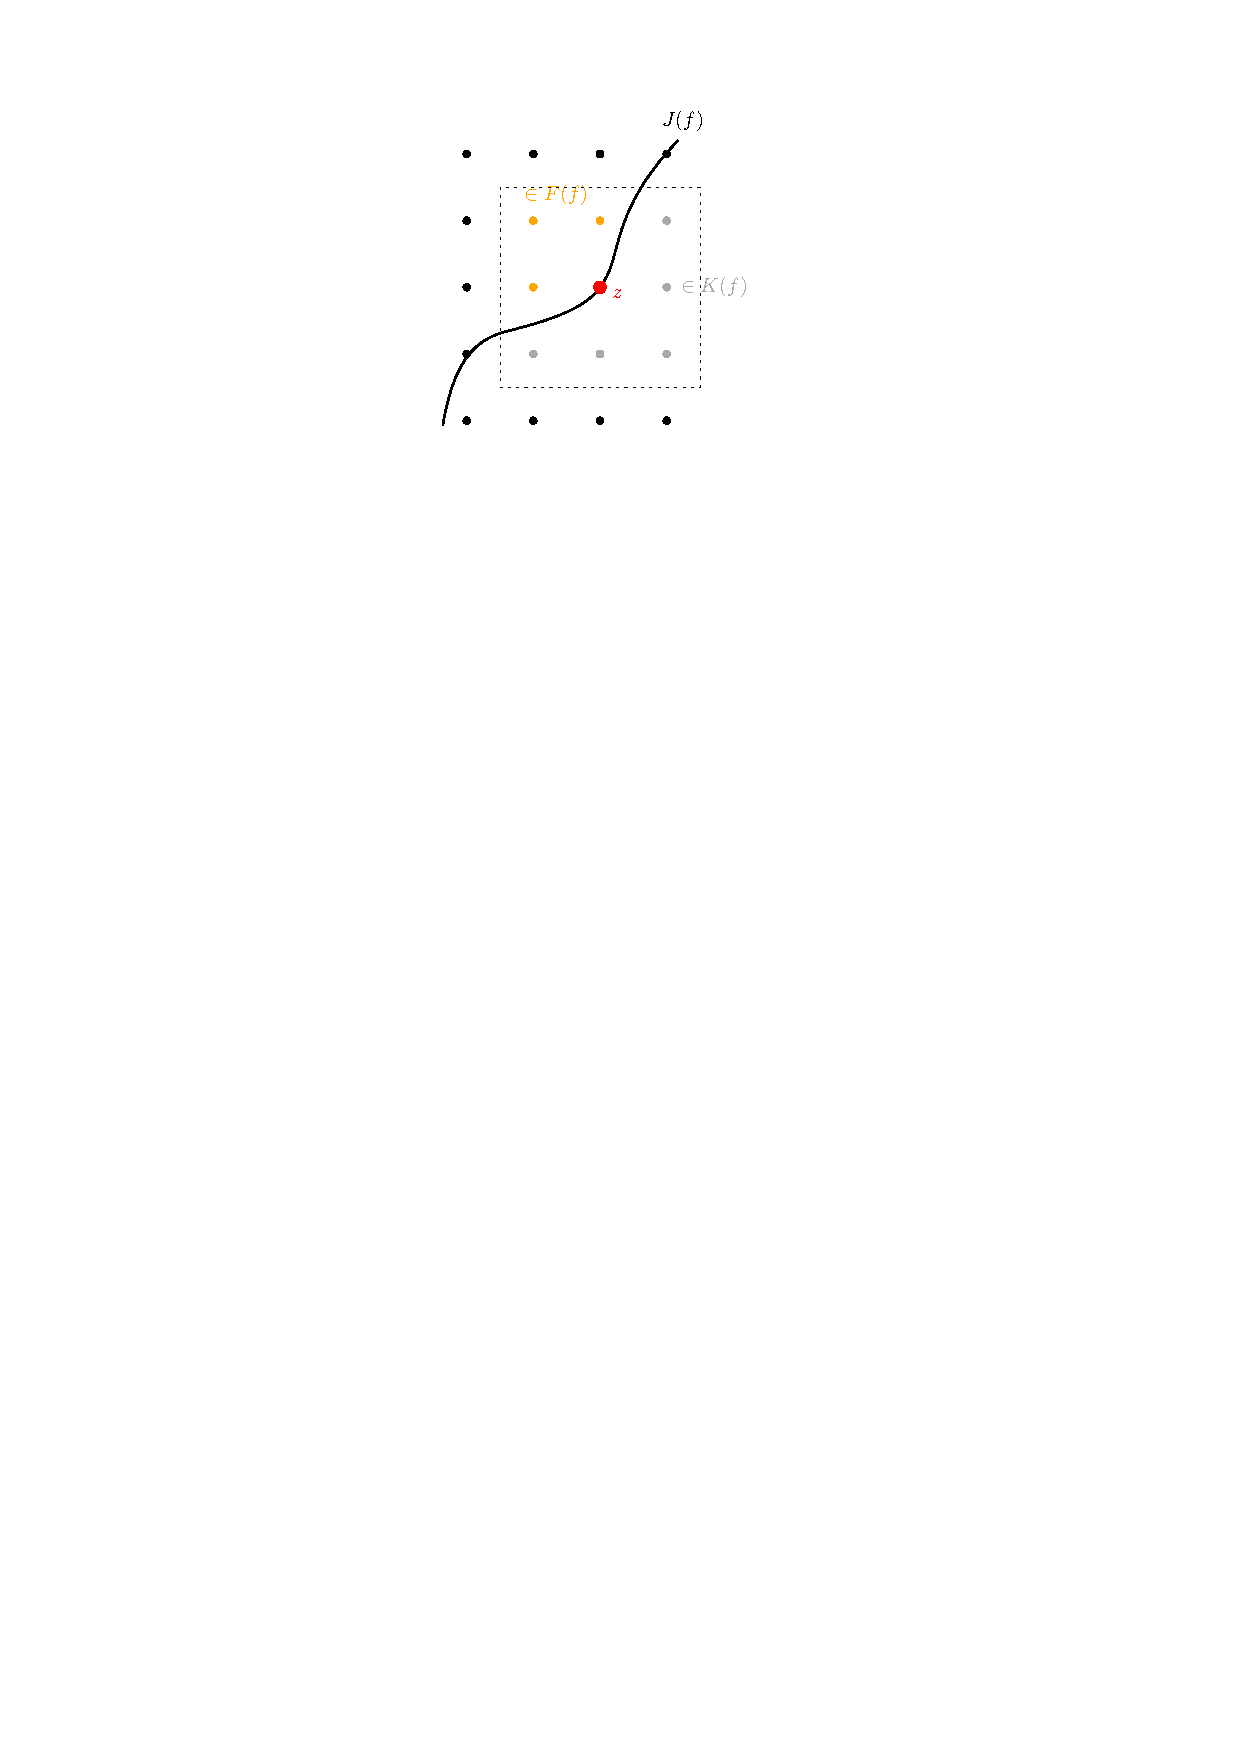
\includegraphics{ch05-hranicni-bod.pdf}
    \caption{Ilustrace hraničního bodu}
    \label{fig:hranicni-bod}
\end{figure}

Na základě této idee si lze již poměrně snad domyslet postup při generování hranice. Pracujeme opět s předpokladem, že oblast komplení roviny představuje diskrétní množinu bodů, které tvoří mřížku (tedy každá dvojice sousedních bodů má stejnou vzdálenost). 
\begin{algorithm}[h]
    \KwIn{Komplexní polynomiální funkce $f$, konečné množiny $X\subset\langle x_{\text{min}},x_{\text{max}}\rangle$ a $Y\subset\langle y_{\text{min}},y_{\text{max}}\rangle$}
    $J\gets\emptyset$\;
    \ForEach{$(x,y)\in X\times Y$}{
        $z\gets x+y\imag$\;
        \If{\textup{existují sousední body $w\in K_\in K(f)$ a $w^\prime\in F(f)$ bodu $z$}}{
            $J\gets J\cup\set{z}$
        }
    }
    \Return{$J$}\;
    \KwOut{Aproximace Juliovy množiny $J$}
    \caption{Generování Juliovy množiny $J$}
    \label{alg:generovani-jf}
\end{algorithm}
\begin{program}
\begin{lstlisting}[style=python]
h_px = len(iter_counts)
w_px = len(iter_counts[0])

# List od inner points
inside = [
    [iter_counts[y][x] == max_iterations for x in range(w_px)]
    for y in range(h_px)
]

# Determine boundary points
boundary_mask = [[False]*w_px for _ in range(h_px)]
for y in range(h_px):
    for x in range(w_px):
        if inside[y][x]:
            for dx, dy in ((1,0),(-1,0),(0,1),(0,-1)):
                nx, ny = x+dx, y+dy
                if 0 <= nx < w_px and 0 <= ny < h_px:
                    if not inside[ny][nx]:
                        boundary_mask[y][x] = True
                        break
\end{lstlisting}
    \caption{Implementace algoritmu \ref{alg:generovani-jf}}
    \label{prog:generovani-jf}
\end{program}

\subsection{Přiřazování barev}\label{subsec:prirazovani-barev}

Jako poslední si pojďme popovídat o barvách a jejich přiřazování jednotlivým bodům. Již jsme měli možnost vidět několik příkladů obrázků s fraktály, kde byly body barevně zvýrazněny. Zevrubně bychom mohli říci, že čím blíž se bod necházel hranici útvaru, tím výraznější byla jeho barva.

\subsubsection{Stručně k barevnému modelu HSV}

Ukážeme si zde celkem dvojici základních možností, jak lze přiřazovat barvy daným bodům. K tomu však budeme potřebovat pracovat s barevným modelem \emph{HSV (Hue, Saturation, Value)}\index{HSV}\index{barevný model}\index{model!barevný}\index{barevný model HSV}. S prominutím si zde opět odpustíme delší vysvětlování a budeme předpokládat, že se čtenář již s modelem HSV někdy setkal (podobně jako např. s RGB nebo s CMYK používaným u tiskáren). Avšak základem, jak název napovídá, je trojice následujících složek:
\begin{itemize}
    \item \textbf{hue} (česky \emph{odstín}),
    \item \textbf{saturation} (česky \emph{saturace}, nebo též \emph{sytost})
    \item a \textbf{value} reprezentující hodnotu jasu (tj. podílu bílé barvy).
\end{itemize}
Celkově tento model vychází přímo z vnímání barev lidským okem. Různé možnosti znázornění HSV modelu si lze prohlédnout na obrázcích \ref{subfig:hsv-valcova-reprezentace} a \ref{subfig:hsv-kuzelova-reprezentace}.
\begin{figure}[h]
    \centering
    \begin{subfigure}{0.45\textwidth}
        \centering
        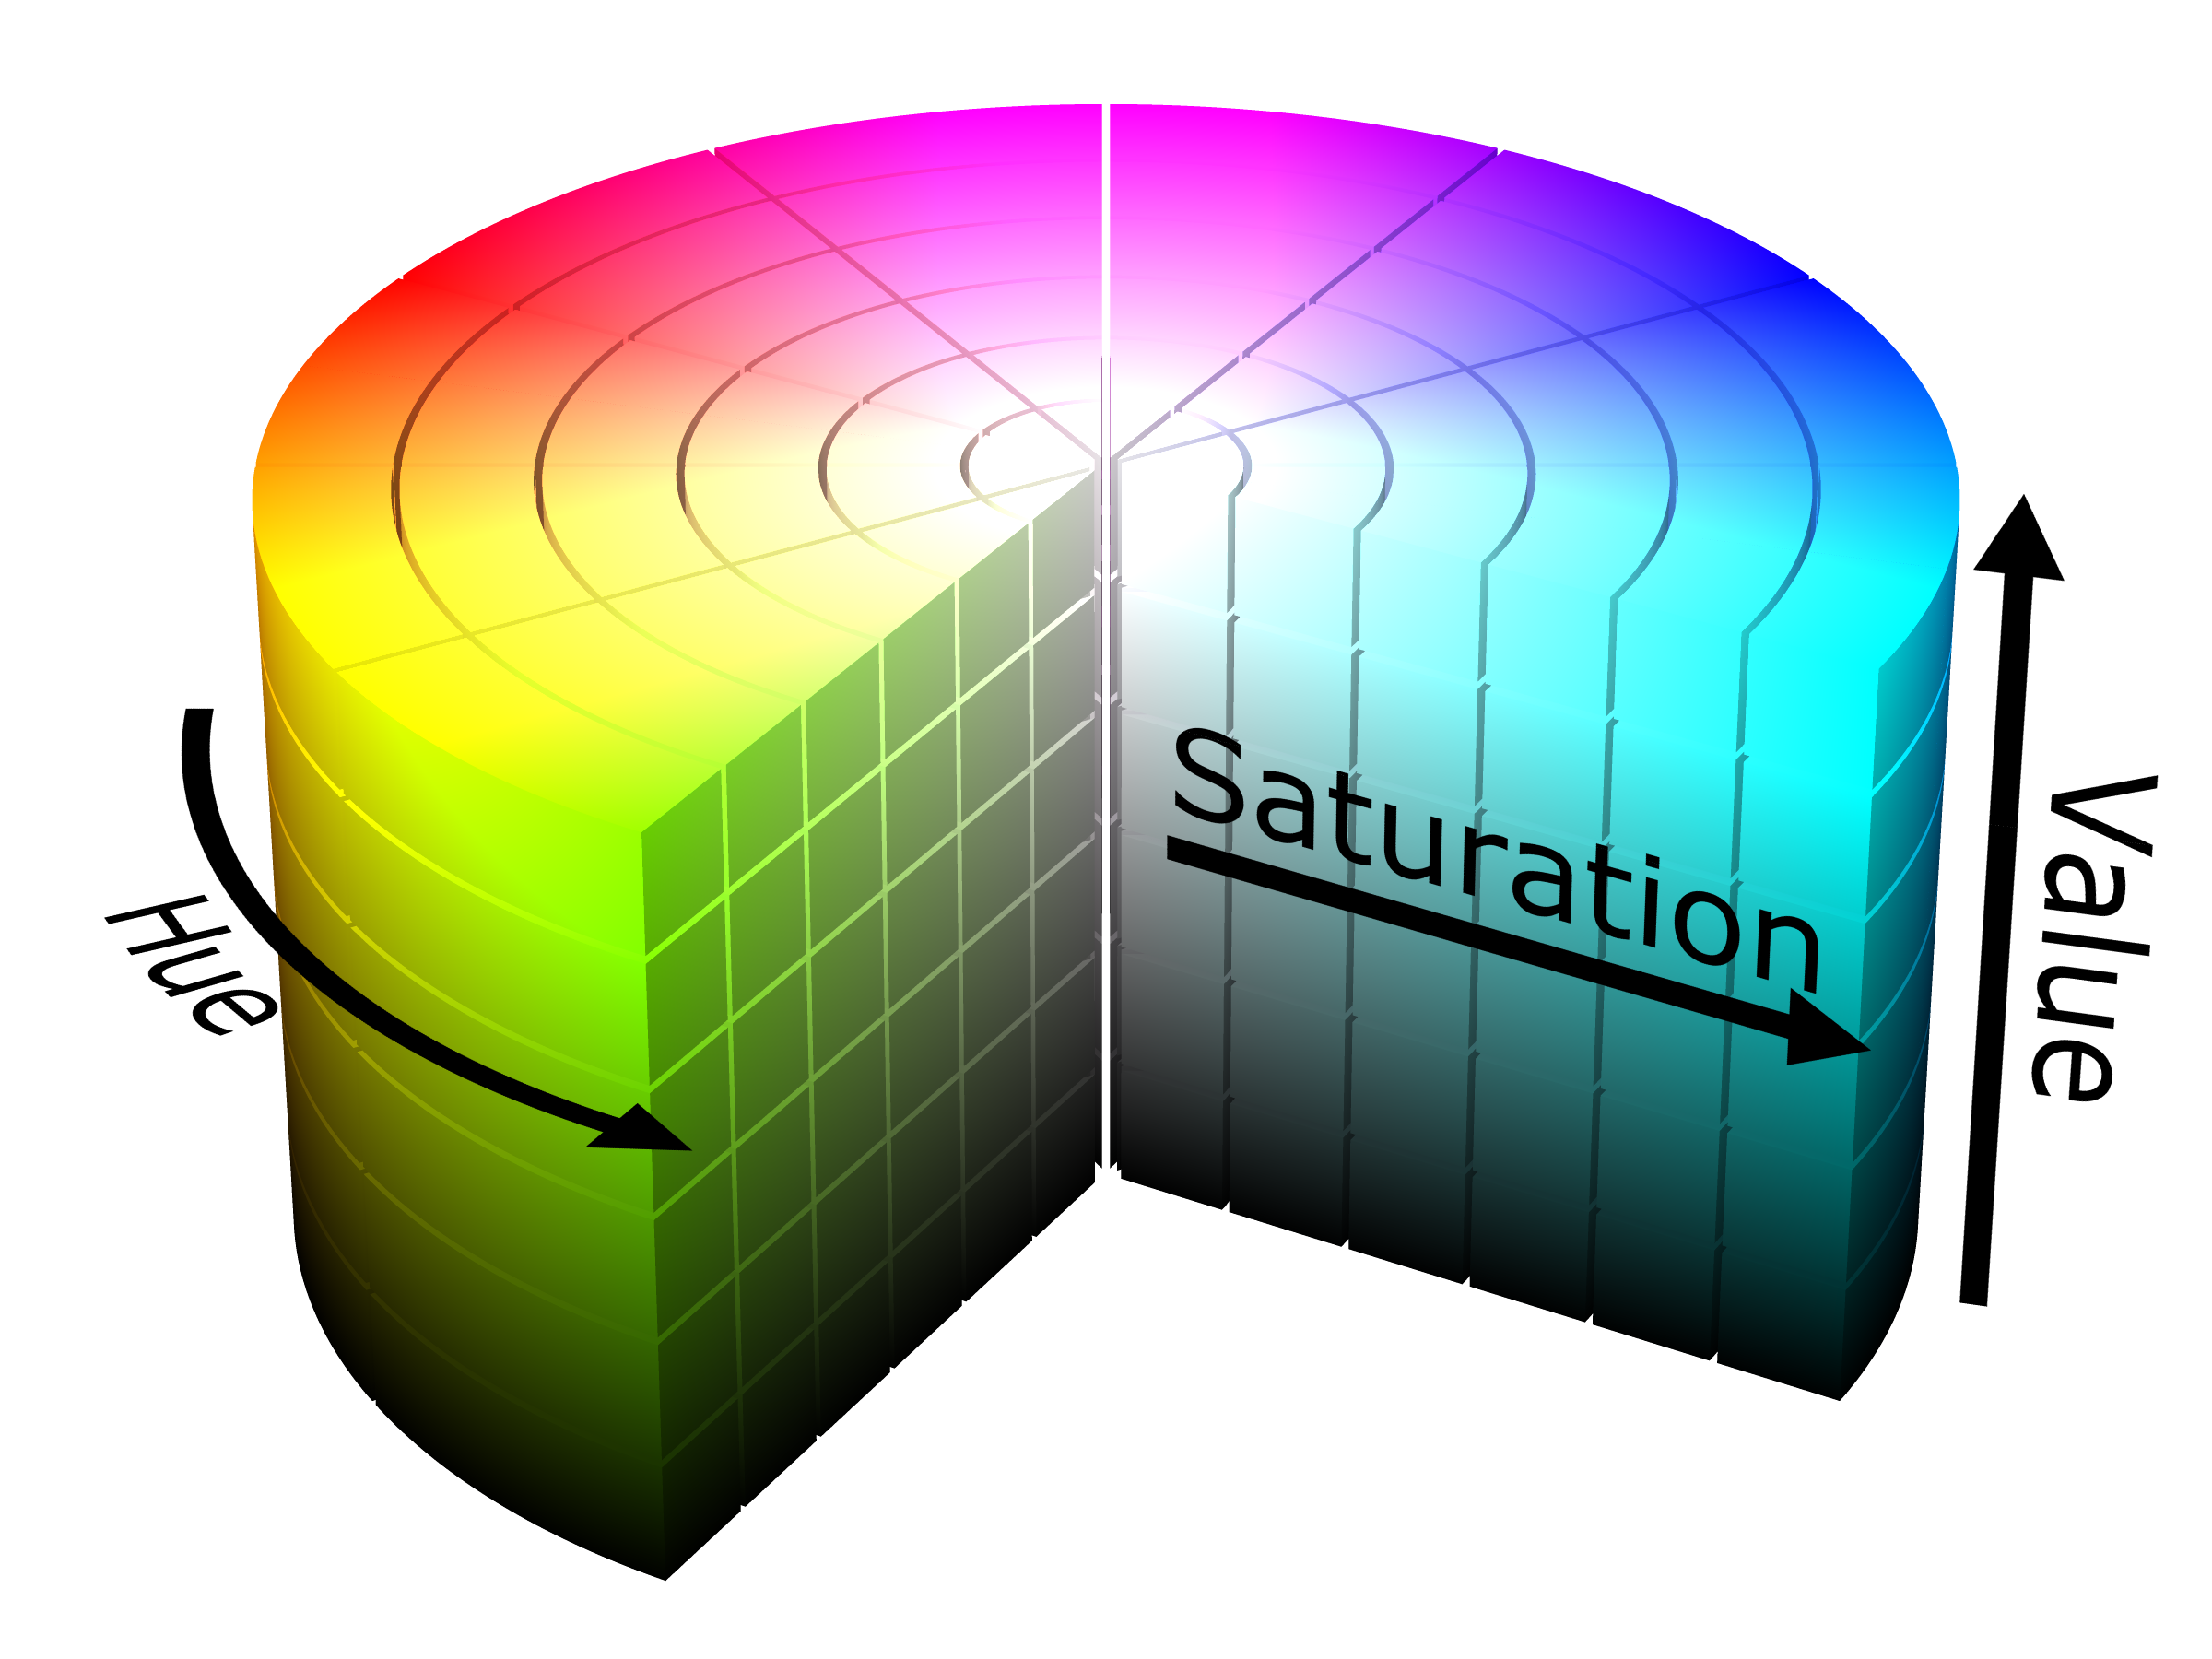
\includegraphics[width=\textwidth]{ch05-HSV_color_solid_cylinder.png}
        \caption{Válcová reprezentace}
        \label{subfig:hsv-valcova-reprezentace}
    \end{subfigure}
    \qquad
    \begin{subfigure}{0.45\textwidth}
        \centering
        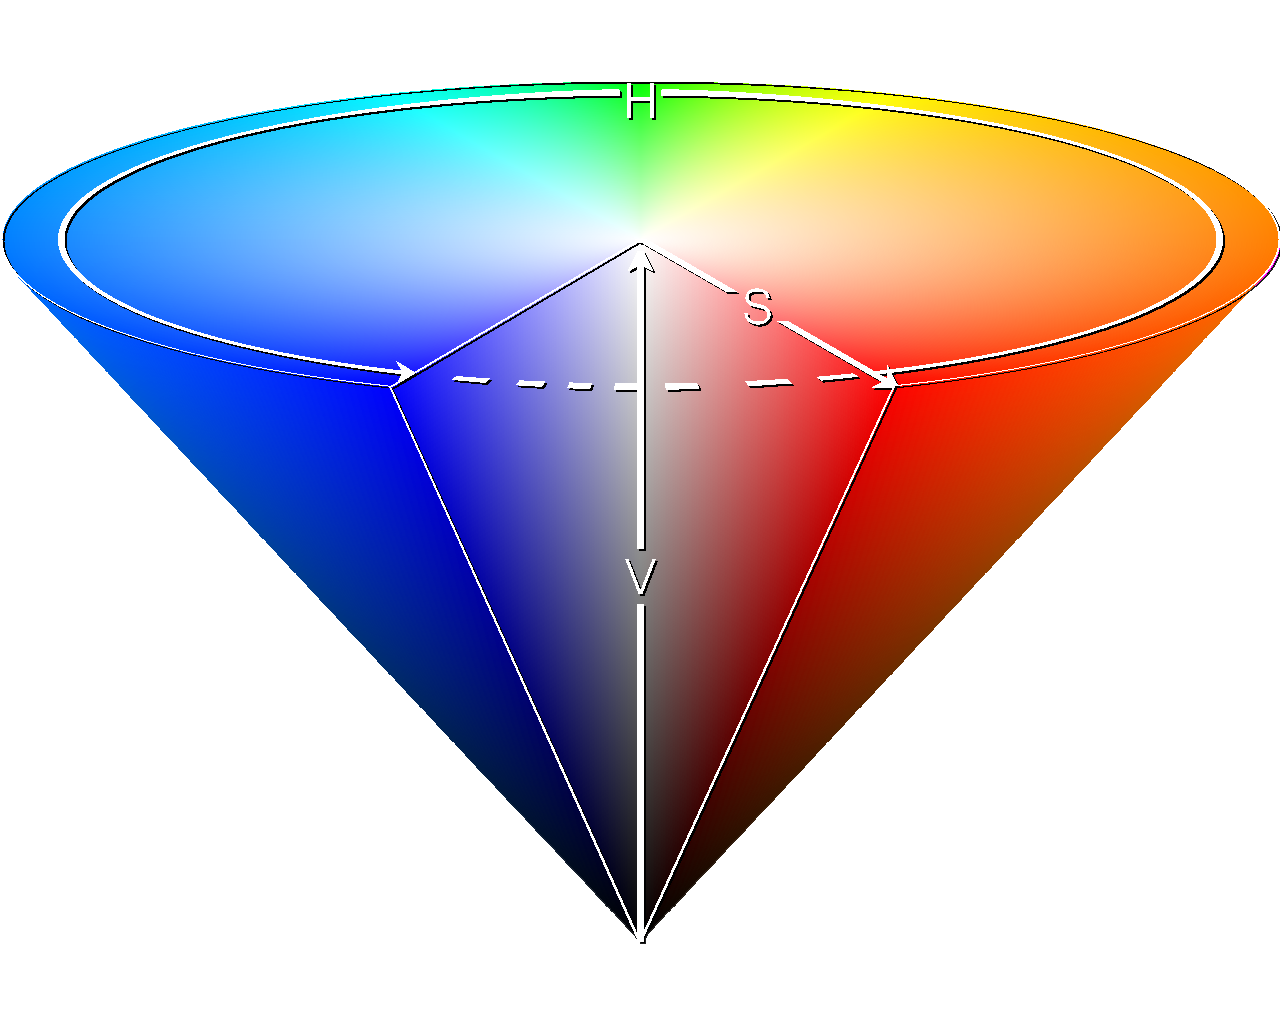
\includegraphics[width=\textwidth]{ch05-HSV_cone.png}
        \caption{Kuželová reprezentace}
        \label{subfig:hsv-kuzelova-reprezentace}
    \end{subfigure}
    \caption[Grafické znázornění HSV modelu]{Grafické znázornění HSV modelu (Převzato z~Wikipedia Commons)\footnotemark}
    \label{fig:hsv}
\end{figure}

Existují pochopitelně metody\footnotetext{Dostupné z \url{https://cs.wikipedia.org/wiki/HSV}} pro převody mezi jednotlivými barevnými modely, ty však pro nás zde nejsou relevantní. Jednotlivé barvy budeme reprezentovat jako uspořádané trojice $(H,S,V)$, kde $0\leqslant H,S,V\leqslant 1$.

\subsubsection{Lineární interpolace barev}

Patrně nejjednodušším způsobem pro přiřazení barev jednotlivým bodům je tzv. \emph{lineární interpolací}\index{lineární interpolace}\index{interpolace!lineární} odstínu při pevně zvolené saturaci a jasu. Obecně jsou-li zadány body v rovině $(x_0,y_0)$ a $(x_1,y_1)$, pak lineární intepolace přiřazuje každému $x\in(x_0,x_1)$ souřadnici $y=f(x)$, takovou, že $(x,y)$ leží na spojnici bodů $(x_0,y_0)$ a $(x_1,y_1)$. Toto lze vyjádřit poměrně jednoduchým vzorcem:
\[f(x)=y_{0}+(x-x_{0}){\frac {y_{1}-y_{0}}{x_{1}-x_{0}}}.\]
Pojďme si nyní rozmyslet náš případ. Bodům z komplexní roviny budeme přiřazovat barvu podle počtu iterací, kterého jsme při výpočtu dosáhli, než začala samotná postupnost iterací funkce divergovat. Zde mohou tedy nastat celkově dva případy. Počet iterací pro pevně zvolený bod $z$ si označme $k$ a maximální počet iterací si označme $m$.
\begin{itemize}
    \item Pokud $k<m$, pak přižadíme bodu $z$ barvu na základě lineární interpolace odstínu, přičemž saturaci a jas volíme pevně, označme $S_0,V_0$.
    \item Pokud $k=m$, pak bodu $z$ přiřadíme černou barvu, tedy prohlásíme jej za bod náležící zkoumané vyplněné Juliově množině.
\end{itemize}

Hodnoty odstínu $H$ nabývají hodnot z intervalu $\langle H_{\text{min}},H_{\text{max}}\rangle$, přičemž
\[0\leqslant H_{\text{min}},H_{\text{max}}\leqslant 1\]
a hodnoty $k$ jsou z množiny $\set{0,1,2,\ldots,m}$. Tedy celkový předpis lineární interpolaci odstínu bude
\[H=H_{\text{min}}+k\cdot\frac{H_{\text{max}}-H_{\text{min}}}{m}\]
a tudíž pro výslednou barvu bodu $z$ bude platit 
\[(H,S,V)=\begin{cases}
    \left(H_{\text{min}}+k(H_{\text{max}}-H_{\text{min}})/m,S_0,V_0\right) & k<m,\\
    (0,0,0) & k=m.
\end{cases}\]
Pro ukázku viz obrázky \ref{fig:mandelbrotova-mnozina-lerp-1} a \ref{fig:mandelbrotova-mnozina-lerp-2} s hranicí Mandebrotovy množiny.
\begin{figure}[h]
    \centering
    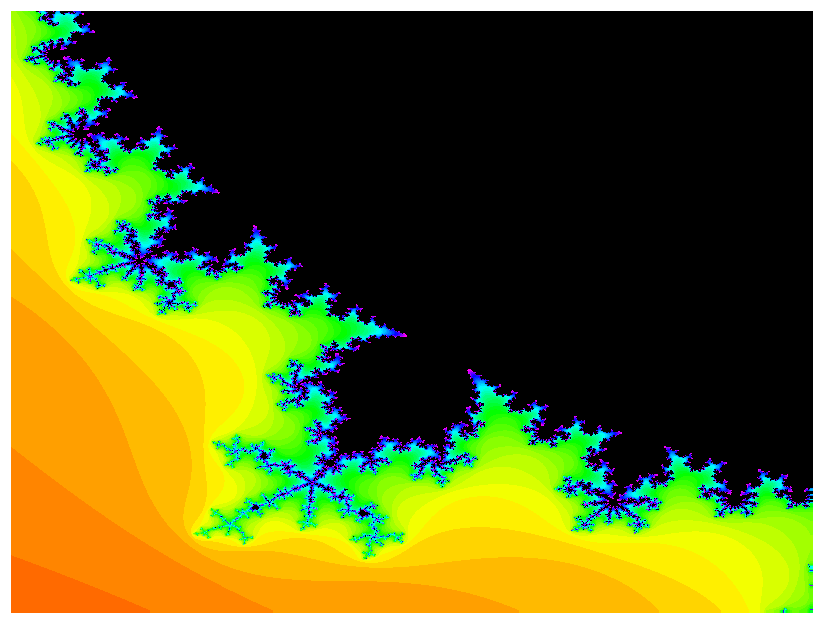
\includegraphics[width=\textwidth]{mandelbrot_set_zoom_1_lerp.png}
    \caption{Mandebrotova množina pomocí lineární interpolace odstínu pro hodnoty $H_{\text{min}}=0;H_{\text{max}}=0{,}87;S_0=V_0=1;m=50$}
    \label{fig:mandelbrotova-mnozina-lerp-1}
\end{figure}
\begin{figure}[h]
    \centering
    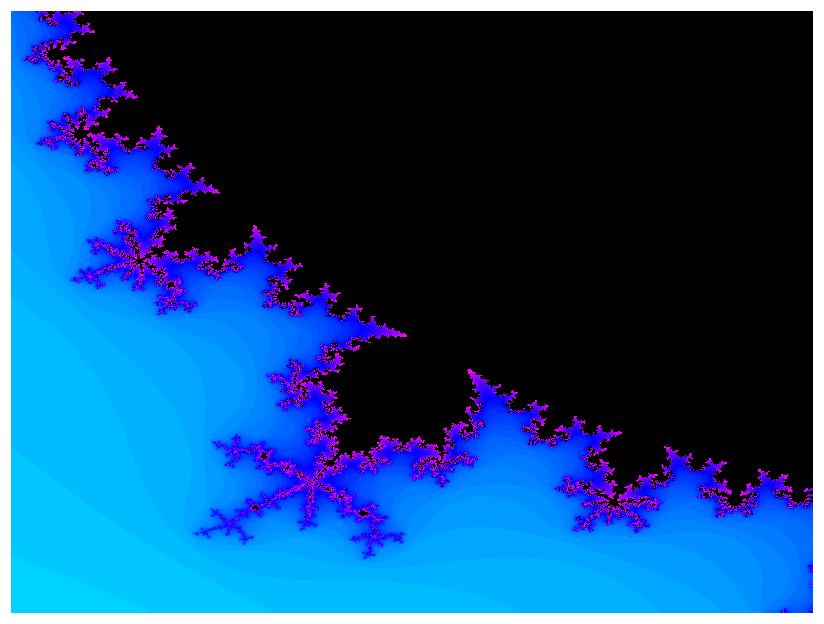
\includegraphics[width=\textwidth]{mandelbrot_set_zoom_1_lerp-2.png}
    \caption{Mandebrotova množina pomocí lineární interpolace odstínu pro hodnoty $H_{\text{min}}=0{,}5;H_{\text{max}}=0{,}861;S_0=1;V_0=0{,}5;m=50$}
    \label{fig:mandelbrotova-mnozina-lerp-2}
\end{figure}

Pochopitelně stejně jako odstín lze interpolovat i zbylé dvě složky. Není třeba se omezovat pouze nutně na odstín.
\begin{align*}
    H&=H_{\text{min}}+k\cdot\frac{H_{\text{max}}-H_{\text{min}}}{m},\\
    S&=S_{\text{min}}+k\cdot\frac{S_{\text{max}}-S_{\text{min}}}{m},\\
    V&=V_{\text{min}}+k\cdot\frac{V_{\text{max}}-V_{\text{min}}}{m}.
\end{align*}
Pokud bychom chtěli využít sofistrikovanější barvení, mohli bychom též využít obecný interpolační polynom. Ten lze např. určit pomocí tzv. \emph{Lagrangeovy interpolace}\index{interpolace!Lagrangeova}\index{Lagrangeova interpolace}, kdy při známých funkčních hodnonách $f(x_0),f(x_1),\ldots,f(x_n)$ pro nazvájem různá $x_0,x_1,\ldots,x_n$ lze sestavit interpolační polynom $L_n(x)$ pomocí vzorce
\[L_n(x)=\sum_{i=0}^{n}f(x_i)\prod_{\substack{0\leqslant j\leqslant n\\j\neq i}}{\frac {x-x_{j}}{x_{i}-x_{j}}}.\]
Lze si všimnout, že takto definovaná funkce $L_n$ prochází všemi zadanými body, protože pro libovolné $x_\ell$, kde $0\leqslant\ell\leqslant n$, platí
\begin{align*}
    L_n(x_\ell)&=\sum_{i=0}^{n}f(x_i)\prod_{\substack{0\leqslant j\leqslant n\\j\neq i}}{\frac {x-x_{j}}{x_{i}-x_{j}}}=\sum_{i=0}^{n}f(x_i)\frac{x_\ell-x_\ell}{x_{\ell}-x_{j}}\prod_{\substack{0\leqslant j\leqslant n\\j\neq i,j\neq\ell}}{\frac {x_\ell-x_{j}}{x_{i}-x_{j}}}\\
    &=\sum_{i=0}^{n}f(x_i)\delta_{i\ell}=f(x_\ell),
\end{align*}
kde $\delta_{ij}$ je Kroneckerovo delta\footnote{Kroneckerovo delta se definuje jako
\[\delta_{ij}=\begin{cases}
    1 & i=j\\
    0 & i\neq j
\end{cases}.\]
}.

\subsubsection{Hladké zbarvení}

Ačkoliv bychom se s výsledkem pomocí prosté lineární interpolace (viz obrázky \ref{fig:mandelbrotova-mnozina-lerp-1} a \ref{fig:mandelbrotova-mnozina-lerp-2}) mohli spokojit, lze si všimnout, že přechody mezi jednotlivými barvami (co by aproximacemi vyplněné Juliovy množiny pro zvolenou polynomiální funkci) jsou velmi ostré. Je tomu tak z důvodu, že ze zvolené lineární interpolace vzniká konečná posloupnost hodnot $H$ (funkce tedy není spojitá). Tento problém bychom mohli vyřešit zvýšením maximálního počtu iterací, tedy v konečném důsledku by mezi barvami nebyly takové rozdíly (pro porovnání s obrázkem \ref{fig:mandelbrotova-mnozina-lerp-1} viz obrázek \ref{fig:mandelbrotova-mnozina-lerp-3}, kde $m=100$).
\begin{figure}[h]
    \centering
    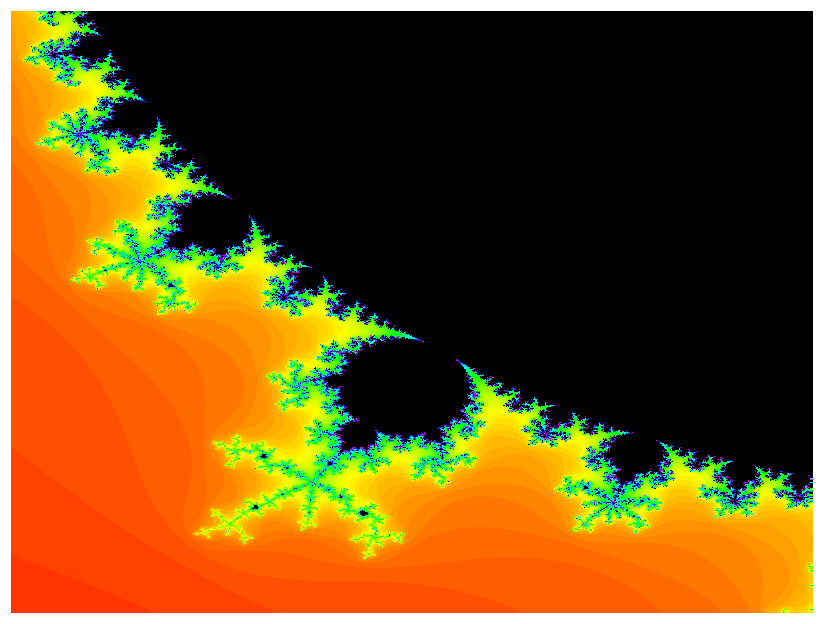
\includegraphics[width=\textwidth]{mandelbrot_set_zoom_1_lerp-3.png}
    \caption{Mandebrotova množina pomocí lineární interpolace odstínu pro hodnoty $H_{\text{min}}=0;H_{\text{max}}=0{,}87;S_0=V_0=1;m=100$}
    \label{fig:mandelbrotova-mnozina-lerp-3}
\end{figure}
Nicméně zvýšením maximálního počtu iterací se podstatně zvyšuje náročnost výpočtu. Zkusme se tedy místo toho více zaměřit na způsob výpočtu výsledného odstínu. Často se při lineární interpolaci nepoužívá přímo počet iterací $k$, nýbrž číslo
\[k_s=k+\dfrac{\log(\log|f^{\circ k}(z)|)}{\log{2}}\]
Tento vzorec si zde nebudeme odvozovat, avšak vychází z tzv. \emph{potenciálové funkce}\index{funkce!potenciálová}\index{potenciálová funkce}, která se definuje jako
\[\varphi(z)=\lim_{k\to \infty }{\frac {\log|f^{\circ k}(z)|}{d^{k}}},\]
kde $d=\deg{f}$.

Díky zohlednění absolutní hodnoty $|f^{\circ k}(z)|$ budou přechody mezi barvami již daleko jemnější. Posuďte sami (viz obrázek \ref{fig:mandelbrotova-mnozina-smooth}).
\begin{figure}[h]
    \centering
    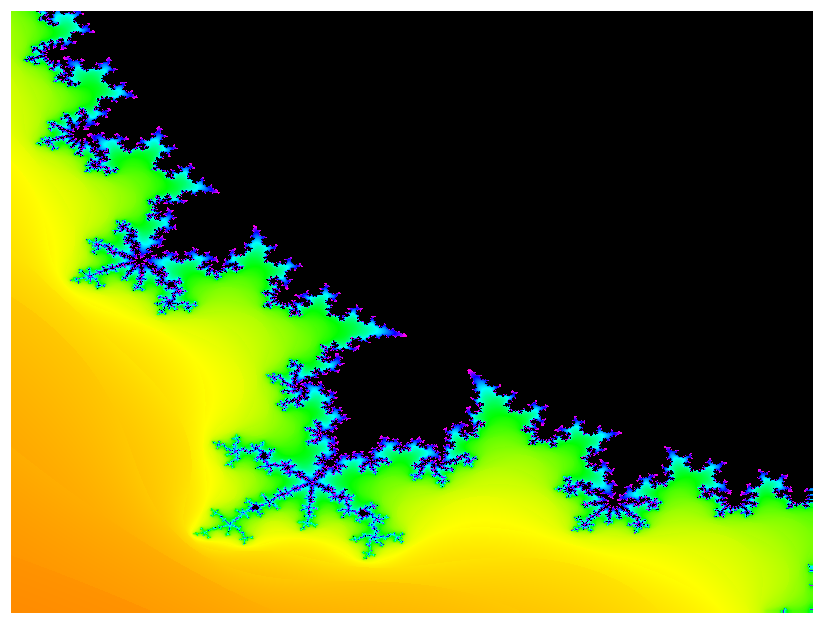
\includegraphics[width=\textwidth]{mandelbrot_set_zoom_1-smooth.png}
    \caption{Mandebrotova množina pomocí hladkého zbarvení pro hodnoty $H_{\text{min}}=0;H_{\text{max}}=0{,}87;S_0=V_0=1;m=50$}
    \label{fig:mandelbrotova-mnozina-smooth}
\end{figure}
